%%%%%%%%%%%%%%%%%%%%%% Generalities %%%%%%%%%%%%%%%%%%5
\documentclass[11pt,fleqn]{amsart}
%\usepackage[paper=a4paper]
 %{geometry}

\pagestyle{plain}
\pagenumbering{arabic}
%%%%%%%%%%%%%%%%%%%%%%%%%%%%%%%%
\usepackage[small]{titlesec}
\usepackage{hyperref}
\usepackage{amsthm,thmtools}
%\usepackage{showlabels}
\linespread{1.05}
%\setlength{\parskip}{1.2ex}

\usepackage[utf8]{inputenc}
\usepackage[english]{babel}
\usepackage{enumerate}
\usepackage[osf,noBBpl]{mathpazo}
\usepackage[alphabetic,initials]{amsrefs}
\usepackage{amsfonts,amssymb,amsmath}
\usepackage{mathtools}
\usepackage{graphicx}
\usepackage[poly,arrow,curve,matrix]{xy}
%\usepackage{wrapfig}
%\usepackage{xcolor}
\usepackage{helvet}
\usepackage{stmaryrd}
\usepackage{tikz}
\usepackage{mathdots}
%\usepackage[normalem]{ulem}

\renewcommand\thesection{\arabic{section}}
\titleformat{\section}
 {\normalfont\bfseries\large}
 {\thesection. \space}{0em}{}

\renewcommand\thesubsection{\arabic{subsection}}
\titleformat{\subsection}
 {\normalfont\bfseries}
 {\thesection.\thesubsection \space}{0em}{}

\renewcommand\proofname{Proof}

\makeatletter
\renewenvironment{proof}[1][\textit{\proofname}]{\par
 \pushQED{\qed}%
 \normalfont \topsep.75\paraskip\relax
 \trivlist
 \item[\hskip\labelsep
 \itshape
 #1\@addpunct{.}]\ignorespaces
}{%
 \popQED\endtrivlist\@endpefalse
}
\makeatother
%%%%%%%%%%%%%%%%%%%%%%%%%%% Theorems et al%%%%%%%%%%%%%%%%%%%%%%%%%%
\declaretheoremstyle[
%headformat=swapnumber, 
bodyfont=\itshape,]{mystyle}
\declaretheorem[name=Lemma, style=mystyle, numberwithin=section]{Lemma}
\declaretheorem[name=Proposition, style=mystyle, sibling=Lemma]{Proposition}
\declaretheorem[name=Theorem, style=mystyle, sibling=Lemma]{Theorem}
\declaretheorem[name=Corollary, style=mystyle, sibling=Lemma]{Corollary}
\declaretheorem[name=Definition, style=mystyle, sibling=Lemma]{Definition}
\declaretheorem[name=Example, style=mystyle, sibling=Lemma]{Example}
\declaretheorem[name=Remark, style=mystyle, sibling=Lemma]{Remark}

% unnumbered versions
\declaretheoremstyle[numbered=no, 
bodyfont=\itshape]{mystyle-empty}
\declaretheorem[name=Lemma, style=mystyle-empty]{Lemma*}
\declaretheorem[name=Proposition, style=mystyle-empty]{Proposition*}
\declaretheorem[name=Theorem, style=mystyle-empty]{Theorem*}
\declaretheorem[name=Corollary, style=mystyle-empty]{Corollary*}
\declaretheorem[name=Definition, style=mystyle-empty]{Definition*}
\declaretheorem[name=Example, style=mystyle-empty]{Example*}
\declaretheorem[name=Remark, style=mystyle-empty]{Remark*}

%%%%%%%%%%%%%%%%%%%%%%%%%%% Paragraphs %%%%%%%%%%%%%%%%%%%%%%%%%%%%%
\newskip\paraskip
\paraskip=0.75ex plus .2ex minus .2ex

\newcounter{para}[section]
\setcounter{para}{0}
\renewcommand\thepara{\thesection.\arabic{para}}
\def\paragraph{%
 \noindent
 \refstepcounter{para}%
 \textbf{\thepara.}\hspace{1ex}%
}

\newcommand\about[1]{%
 {\bfseries#1.}%
}

\newcommand\pref[1]{\textbf{\ref{#1}}}

\renewcommand\theHpara{\theHsection.\arabic{para}}
%%%%%%%%%%%%%%%%%%%%%%%%%%% The usual stuff%%%%%%%%%%%%%%%%%%%%%%%%%
\newcommand\NN{\mathbb N}
\newcommand\CC{\mathbb C}
\newcommand\QQ{\mathbb Q}
\newcommand\RR{\mathbb R}
\newcommand\ZZ{\mathbb Z}
\renewcommand\k{\Bbbk}

\newcommand\maps{\longmapsto}
\newcommand\ot{\otimes}
\renewcommand\to{\longrightarrow}
\renewcommand\phi{\varphi}
\newcommand\id{\mathsf{Id}}
\newcommand\im{\mathsf{im}}
\newcommand\coker{\mathsf{coker}}
%%%%%%%%%%%%%%%%%%%%%%%%% Specific notation %%%%%%%%%%%%%%%%%%%%%%%%%
%\newcommand\II{\mathcal I}
%\newcommand\II'{\mathcal J}

\newcommand\g{\mathfrak g}
\newcommand\p{\mathfrak p}
\newcommand\m{\mathfrak m}
\newcommand\gl{\mathfrak{gl}}
\newcommand\vv{\overline{v}}
\newcommand\II{\mathbb I}
\newcommand\RI{\overline{\mathbb I}}

\newcommand\vectspan[1]{\left\langle #1 \right\rangle}
\newcommand\interval[1]{\llbracket #1 \rrbracket}
\newcommand\abs[1]{|#1|}

\DeclareMathOperator\Frac{Frac}
\DeclareMathOperator\Specm{Specm}
\DeclareMathOperator\End{End}
\DeclareMathOperator\Hom{Hom}

\DeclareMathOperator\sym{sym}
\DeclareMathOperator\asym{asym}
\DeclareMathOperator\sg{sg}
\DeclareMathOperator\ev{\mathsf{ev}}
\DeclareMathOperator\supp{supp}

\newcommand\DD{\mathbb D}
\newcommand\D{\mathfrak D}
\newcommand\bigmodule{big GT module~}

\renewcommand\labelitemi{--}

%%%%%%%%%%%%%%%%%%%%%%%%%%%%%%%%%%%%%% TITLES %%%%%%%%%%%%%%%%%%%%%%%%%%%%%%
\title{Children of big Gelfand-Tsetlin modules}
%\author{[structure.tex]}
\date{}


\begin{document}
\maketitle
%\vspace{-2cm}
\section{Combinatorial preliminaries}

\paragraph
\about{Notation}
\label{notation}
Given $a,b,k \in \NN$ we set $\interval{a,b} = \{i \in \NN \mid a \leq i \leq 
b\}$ and $\interval{b} = \interval{1,b}$. Also we denote by $S_k$ the 
symmetric group in $k$-elements, and given $\pi = (\pi_1, \ldots, \pi_r)$
with $\sum_i \pi_i = k$ we denote by $S_\pi$ the product of symmetric groups
$S_{\pi_1} \times S_{\pi_2} \times \cdots \times S_{\pi_r}$, seen in the 
natural way as subgroup of $S_k$.

Fix $n \in \NN$ and let $\mu = (1, 2, \ldots, n)$. Given $\sigma \in S_\mu$ we 
write $\sigma_{(k)}$ for its projection to $S_k$. We make a slight abuse of 
notation, and identify $S_k$ with the subgroup of $S_\mu$ consisting of 
elements such that $\sigma_(i)$ is the identity for all $i \neq k$. Thus we 
can write $\sigma = \sigma_{(1)} \sigma_{(2)} \cdots \sigma_{(n)}$.

The group $S_\mu$ is a Coxeter group with generating set $\{(i,i+1)_{(k)}
\mid k \in \interval{n}, i \in \interval{k-1}\}$. The usual notions of length,
Bruhat order, parabolic subgroups, etc. will be considered with respect to 
this generating set. In particular the length of $\sigma \in 
S_\mu$ is equal to $\ell_1(\sigma_{(1)}) + \ell_2(\sigma_{(2)}) + \cdots + 
\ell_n(\sigma_{(n)})$, where $\ell_k$ is the usual notion of length in $S_k$.
Also $\sigma < \tau$ in the strong or weak Bruhat order if and only if 
$\sigma_{(k)} < \tau_{(k)}$ for all $k$.

Set $\Sigma = \{(k,i) \mid 1 \leq i \leq k \leq n\}$. The group $S_\mu$ acts 
on $\Sigma$ with the action giben by $\sigma \cdot (k,i) = (k, 
\sigma_{(k)}(i))$. The subset $\Sigma' = \{(k,i) \mid 1 \leq i \leq k \leq n-1
\}$ is clearly invariant by this action. 

Given $a \leq b \leq k$ we set $\interval{a,b}_k = \{(k,i) \mid i \in 
\interval{a,b}\} \subset \Sigma$. Such a set will be called an \emph{interval}
of $\Sigma$, and given an interval $I = \interval{a,b}_k$ we write $a(I) = a,
b(I) = b, k(I) = k$. A partition of $\Sigma$ is a family of nonempty subsets 
of $\Sigma$, which we cal \emph{blocks}, whose disjoint union is $\Sigma$.
An \emph{interval partition} is a partition $\II$ whose blocks are intervals. 
We write $\II[k]$ for the set of all intervals $I \in \II$ with $k(I) = k$. 
We denote by $S(\II)$ the subgroup of $S_\mu$ stabilizing the blocks of $\II$,
which is a parabolic subgroup of $S_\mu$.

\paragraph
Let $\CC^\mu = \CC \times \CC^2 \times \cdots \times \CC^n$, so $v \in \CC^\mu$
is an $n$-tuple $(v_1, v_2, \ldots, v_n)$ with $v_k = (v_{k,1}, v_{k,2},
\ldots, v_{k,k}) \in \CC^k$. For each $(k,i) \in \Sigma$ we denote by 
$\delta^{k,i} \in \CC^\mu$ the unique element in $\CC^\mu$ such that 
$\delta^{k,i}_{l,j} = \delta_{k,l} \delta_{i,j}$, and refer to the set 
$\{\delta^{k,i}\mid (k,i) \in \Sigma\}$ as the canonical basis of $\CC^\mu$. 
The group $S_\mu$ acts on $\CC^\mu$ by linear operators whose action on the 
canonical basis is given by $\sigma \cdot \delta^{k,i} = \delta^{\sigma \cdot 
(k,i)} = \delta^{k, \sigma_{(k)} (i)}$. We denote by $\ZZ^\mu_0$ the abelian 
group generated by $\{\delta^{k,i} \mid 1 \leq i \leq k \leq n-1\}$, which is 
clearly stable by the action of $S_\mu$.

Given $v \in \CC^\mu$ we construct a graph $\Omega(v)$ as follows. The set of 
vertices of $\Omega(v)$ is $\{[k,i] \mid (k,i) \in \Sigma\}$, and we have an 
edge between $[k,i]$ and $[l,j]$ if and only if $v_{k,i} - v_{l,j} \in \ZZ$ 
and $\abs{k-l} \leq 1$. We will write $[k,i] - [l,j]$ as an abbreviation of 
``the edge between $[k,i]$ and $[l,j]$'' (we use square brackets to denote 
vertices so there is less chance of confusing the vertex with a minus). We say 
two vertices are connected if they lie in the same connected component of 
$\Omega(v)$. 

Given an interval $I = \interval{a,b}_k$ we will write $v(I)$ for $(v_{k,a}, 
v_{k,a+1}, \cdots, v_{k,b})$. Given an interval partition $\II$ of $\Sigma$ we 
refer to the tuples $v(I)$ with $I \in \II$ as the $\II$-blocks of $v$. We 
associate with $v$ a partition of $\Sigma$ denoted by $\II(v)$, where the 
block of $(n,i)$ is $\{(n,i)\}$, and for $k < n$ the block of $(k,i)$ is the 
set of all $(k,j)$ such that $[k,i] - [k,j]$ is an edge in $\Omega(v)$.

\begin{Definition}
We say that $v \in \CC^\mu$ is in \emph{normal form} if $[k,a] - [k,b]$
and $a < b$ implies that $v_{k,i} - v_{k,j} \in \ZZ_+$ for all $i,j \in 
\interval{a,b}$ with $i < j$. 
\end{Definition}
Clearly for each $v \in \CC^\mu$ there exists at least one element in its 
$S_\mu$-orbit which is in normal form. 

Suppose $v$ is in normal form and let $\II(v)[k] = \{I_1, I_2, \ldots, I_r\}$, 
with $a(I_i) = b(I_{i-1}) + 1$. We set $\pi(v,k) = (\abs{I_1},\abs{I_2}, 
\ldots, \abs{I_r})$, so $S_{\pi(v,k)}$ is a parabolic subgroup of $S_k$; 
observe that by definition $S_{\pi(v,n)}$ is the trivial subgroup of $S_n$. 
We denote by $\pi(v)$ the concatenation of $\pi(v,1), \pi(v,2), \ldots,
\pi(v,n)$, and set $S_{\pi(v)} = S_{\pi(v,1)} \times S_{\pi(v,2)} \cdots 
\times S_{\pi(v,n)} \subset S_\mu$, which a parabolic subgroup of $S_\mu$.
\begin{Definition}
We say that $\vv \in \CC^\mu$ is a \emph{seed} if it is in normal form and 
$v_{k,i} = v_{l,j}$ whenever $[k,i]$ and $[l,j]$ are connected in $\Omega(v)$.
\end{Definition}
It follows that for every $v \in \CC^\mu$ there exists $z \in \ZZ^\mu_0$ such
that $\vv = v + z$ is a seed.
\begin{Example}
We will write elements of $\CC^\mu$ as triangular arrays with $k$ entries in
its $k$-th row. In this and all other examples we assume that the set $\{1, a,
b, c, \ldots\} \subset \CC$ is linearly independent over $\ZZ$.

\begin{tabular}{cc}
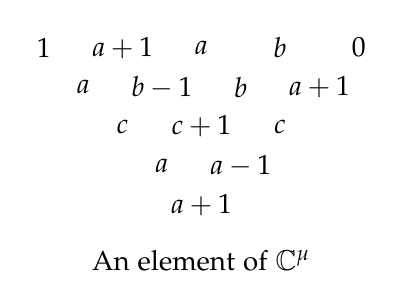
\begin{tikzpicture}
\node (51) at (-2,2.5) {$1$};
\node (52) at (-1,2.5) {$a+1$};
\node (53) at (0,2.5) {$a$};
\node (54) at (1,2.5) {$b$};
\node (55) at (2,2.5) {$0$};

\node (41) at (-1.5,2) {$a$};
\node (42) at (-0.5,2) {$b-1$};
\node (43) at (0.5,2) {$b$};
\node (44) at (1.5,2) {$a+1$};

\node (31) at (-1,1.5) {$c$};
\node (32) at (0,1.5) {$c+1$};
\node (33) at (1,1.5) {$c$};

\node (21) at (-.5,1) {$a$};
\node (22) at (.5,1) {$a-1$};

\node (11) at (0,0.5) {$a+1$};

\node (text) at (0,-0.2) {An element of $\CC^\mu$};
\end{tikzpicture}

&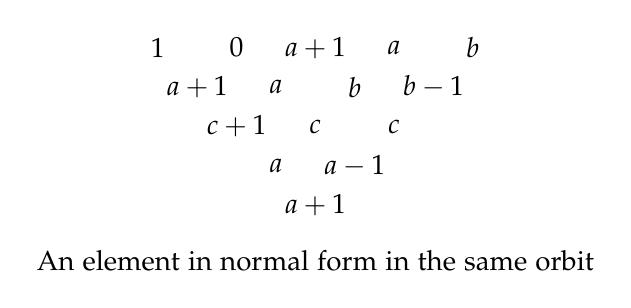
\begin{tikzpicture}
\node (51) at (-2,2.5) {$1$};
\node (52) at (-1,2.5) {$0$};
\node (53) at (0,2.5) {$a+1$};
\node (54) at (1,2.5) {$a$};
\node (55) at (2,2.5) {$b$};

\node (41) at (-1.5,2) {$a+1$};
\node (42) at (-0.5,2) {$a$};
\node (43) at (0.5,2) {$b$};
\node (44) at (1.5,2) {$b-1$};

\node (31) at (-1,1.5) {$c+1$};
\node (32) at (0,1.5) {$c$};
\node (33) at (1,1.5) {$c$};

\node (21) at (-.5,1) {$a$};
\node (22) at (.5,1) {$a-1$};

\node (11) at (0,0.5) {$a+1$};

\node (text) at (0,-0.2) {An element in normal form in the same orbit};
\end{tikzpicture} \\

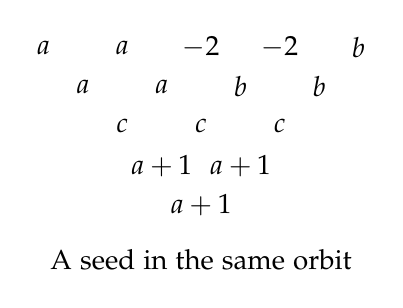
\begin{tikzpicture}
\node (51) at (-2,2.5) {$a$};
\node (52) at (-1,2.5) {$a$};
\node (53) at (0,2.5) {$-2$};
\node (54) at (1,2.5) {$-2$};
\node (55) at (2,2.5) {$b$};

\node (41) at (-1.5,2) {$a$};
\node (42) at (-0.5,2) {$a$};
\node (43) at (0.5,2) {$b$};
\node (44) at (1.5,2) {$b$};

\node (31) at (-1,1.5) {$c$};
\node (32) at (0,1.5) {$c$};
\node (33) at (1,1.5) {$c$};

\node (21) at (-.5,1) {$a+1$};
\node (22) at (.5,1) {$a+1$};

\node (11) at (0,0.5) {$a+1$};

\node (text) at (0,-0.2) {A seed in the same orbit};
\end{tikzpicture}
&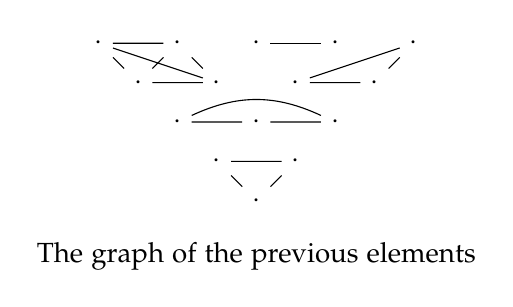
\begin{tikzpicture}
\node (51) at (-2,2.5) {$\cdot$};
\node (52) at (-1,2.5) {$\cdot$};
\node (53) at (0,2.5) {$\cdot$};
\node (54) at (1,2.5) {$\cdot$};
\node (55) at (2,2.5) {$\cdot$};

\node (41) at (-1.5,2) {$\cdot$};
\node (42) at (-0.5,2) {$\cdot$};
\node (43) at (0.5,2) {$\cdot$};
\node (44) at (1.5,2) {$\cdot$};

\node (31) at (-1,1.5) {$\cdot$};
\node (32) at (0,1.5) {$\cdot$};
\node (33) at (1,1.5) {$\cdot$};

\node (21) at (-.5,1) {$\cdot$};
\node (22) at (.5,1) {$\cdot$};

\node (11) at (0,0.5) {$\cdot$};

\node (text) at (0,-0.2) {The graph of the previous elements};

\draw (51) -- (52) -- (42) -- (41) -- (51) -- (42) (52) -- (41);
\draw (53) -- (54);
\draw (55) -- (43) -- (44) -- (55);
\draw (31) -- (32) -- (33) to[out=155,in=25] (31);
\draw (11) -- (21) -- (22) -- (11);
\end{tikzpicture}
\end{tabular}
\end{Example}

\paragraph
\label{descending-z}
\about{Descending $\II$-sequences}
Recall that we denote by $\ZZ^\mu_0$ the set of all $z \in \CC^\mu$ with
$z_{k,i} \in \ZZ$ for all $(k,i) \in \Sigma'$ and $z_{n,i} = 0$ for all $n$.
\begin{Definition}
Let $\II$ be an interval partition of $\Sigma$. We denote by $\DD(\II)$ the 
set of all $z \in \ZZ^\mu_0$ such that $z(I)$ is a decreasing sequence for all 
$I \in \II$. If $\vv$ is a seed we write $\DD(\vv)$ for $\DD(\II(\vv))$.
\end{Definition}
We will only be interested in the case where $\II$ arises as the partition 
associated to a seed, so for the rest of this section we fix a seed $\vv$ and
set $\II = \II(v)$ and $\pi = \pi(v)$.

Let $z \in \DD(\vv)$. The stabilizer of $z$ in $S_\pi$ is again a parabolic 
subgroup of $S_\pi$, which we denote as usual by $(S_\pi)_z$. Thus each 
coclass in $S_\pi/(S_\pi)_z$ has a unique minimal length element, usually 
called a shuffle. We denote by $S_\pi^z$ the set of these minimal length 
representatives, and refer to them as \emph{$z$-shuffles}. Given $\sigma \in
S_\pi$ we denote by $\sigma^z$ the unique $z$-shuffle in $\sigma S_\pi$.

We denote by $\II(\vv,z)$ the interval partition of $\Sigma$ where block of
$(k,i)$ consits of those $(k,j)$ connected to $(k,i)$ in $\Omega(v)$ and such
that $z_{k,i} = z_{k,j}$. Notice that $(S_\pi)_z = S(\II(\vv, z))$. Let 
us say that $\sigma \in S_\pi$ is increasing over an interval 
$\interval{a,b}_k \subset \Sigma$ if $\sigma_{(k)}(i) < \sigma_{(k)}(j)$ 
whenever $a \leq i < j \leq b$. A permutation is a $z$-shuffle if and only if 
it is increasing over every interval in $\II(\vv, z)$, so $\sigma^z$ is the 
unique permutation in $S_\pi$ increasing over all intervals in $\II(\vv, z)$ 
and such that $\sigma^z(z) = \sigma(z)$.

Given an interval $I = \interval{a,b}_k$ we denote by $\omega(I)$ the 
permutation $i \mapsto  b+a-i$. This is the longest element in the symmetric
group of the interval $I$. We also write $\alpha(I)$ for the cyclic 
permutation $(b \ b-1 \ \cdots a)_{(k)}$ and $\beta(I)$ for its inverse, 
namely $(a \ a+1 \ \cdots b)_{(k)}$. It follows that if $\II$ is an interval 
partition then the longest element in $S(\II)$ is $\prod_{I\in\II} \omega(I)$.
\begin{Lemma}
\label{L:omega-delta}
Let $z\in \DD(\vv)$ and let $\omega_0$ be the longest element in $S_\pi$.
\begin{enumerate}[(a)]
\item 
\label{i:omega-z}
We have $\omega_0^z = \omega_0 \prod_{I \in \II(\vv, z)} \omega(I)$.

\item 
\label{i:D-delta}
We have $z + \delta^{k,i} \in \DD(\vv)$ if and only if $i = a(I)$ for some $I 
	\in \II(\vv,z)[k]$. Analogously, $z - \delta^{k,i} \in \DD(\vv)$ if and 
	only if $i = b(I)$ for some $I \in \II(\vv,z)[k]$.

\item 
\label{i:omega-delta}
Let $I \in \II(\vv,z)[k]$. If $z_{k,a(I)-1} \neq z_{k,a(I)} + 1$ then 
	$\omega_0^{z + \delta^{k,a(I)}} = \omega_0^z \alpha(I)$. Analogously,
	if $z_{k,b(I)+1} \neq z_{k,b(I)} - 1$ then $\omega_0^{z - \delta^{k,b(I)}} 
	= \omega_0^z \beta(I)$.
\end{enumerate}
\end{Lemma}
\begin{proof}
Put $\II = \II(\vv,z)$.
By definition $\omega_0$ reverses the order of each interval $J$ in $\II$. In
particular it is decreasing over each interval $I$ contained in any $J$. Since 
$\omega_0(I)$ is decreasing over$I$, it follows that $\omega_0 \prod_{I \in 
\II} \omega(I)$ is increasing over every interval $I \in \II$, so it is a 
$z$-shuffle lying in the coclass $\omega_0 (S_\pi)_z$. This proves item 
\ref{i:omega-z}. Item \ref{i:D-delta} follows immediately from the 
definitions. 

Suppose we are in the first case of item \ref{i:omega-delta} and set $y = z + 
\delta^{k,i}$. Notice first that $\omega(\interval{a(I)+1,b(I)}_k) = 
\omega(I) \alpha(I)$. The hypothesis implies that $\II(\vv,y)[l] = \II[l]$ for 
$l \neq k$, while 
\[
\II(\vv,y)[k] = (\II[k] \setminus I) \cup \{\{(k,a(I))\},
\interval{a(I)+1,b(I)}_k\},
\] 
so by item \ref{i:omega-z}
\begin{align*}
\omega_0^y 
	&= \prod_{J \in \II(\vv,y)} \omega(J)
	= \left(\prod_{J \in \II; J \neq I} \omega(J)\right) 
		\omega(\interval{a(I)+1,b(I)}_k) \\
	&= \left(\prod_{J \in \II} \omega(J)\right)\alpha(I)
	= \omega_0^z \alpha(I).
\end{align*}
The second case of this item is proved similarly.
\end{proof}

\section{Big Gelfand-Tsetlin modules and their submodules}
Throughout this section we fix a seed $\vv$ and set $\II = \II(\vv), \pi = 
\pi(\vv)$.

\paragraph
\about{Gelfand-Tsetlin modules}
For each $k \in \interval{n}$ we denote by $U_k$ the enveloping algebra of 
$\gl(k,\CC)$, and set $U = U_n$. Inclusion of matrices in the top left corner 
induces a chain
\begin{align*}
\gl(1,\CC) \subset \gl(2, \CC) \subset \cdots \subset \gl(n,\CC),
\end{align*}
which in turn induces a chain $U_1 \subset U_2 \subset \cdots \subset U_n$. 
Denote by $Z_k$ the center of $U_k$ and by $\Gamma$ the subalgebra of $U$ 
generated by $\bigcup_{k=1}^n Z_k$. This algebra is the \emph{Gelfand-Tsetlin} 
subalgebra of $U$, and it is generated by the elements
\begin{align*}
c_{k,i}
  &= \sum_{(r_1, \ldots, r_i) \in \interval{k}^i} 
    E_{r_1, r_2} E_{r_2, r_3} \cdots E_{r_i, r_1},
  & (k,i) \in \Sigma(\mu).
\end{align*}
By work of Zhelobenko there exists an isomorphism $c \in \Gamma \to \gamma_c
\in \CC[x_{k,i} \mid (k,i) \in \Sigma]^{S_\mu}$, given by $c_{k,i} mapsto 
\gamma_{k,i}$ where
\begin{align*}
\gamma_{k,i}
  &= \sum_{j=1}^k (x_{k,j} + k - 1)^i 
    \prod_{m \neq j} \left( 
      1 - \frac{1}{x_{k,j} - x_{k,m}}
    \right),
\end{align*}
see \cite{FGR16}*{Subsection 3.1} for details. 
It follows that $\Specm \Gamma \cong \CC^\mu / S_\mu$, and so every 
$v \in \CC^\mu$ induces a character $\chi_v: \Gamma \to \CC$ by setting
$c \in \Gamma \mapsto \gamma_c(v)$. 
\begin{Definition*}
A $U$-module $M$ is called a \emph{Gelfand-Tsetlin module} if it is finitely
generated and
\[
  M = \bigoplus_{\m \in \Specm \Gamma} M[\mathfrak m],
\] 
where $M[\mathfrak m] = \{x \in M \mid \mathfrak m^k x = 0 \mbox{ for some } k 
\geq 0\}$.
\end{Definition*}
Let $M$ be a Gelfand-Tsetlin module and let $v \in \CC^\mu$. We put
$M[v] = M[\ker \chi_v]$, and denote by $p_v: M \to M[v]$ the natural projection
map. We say that $\chi_v$ is a Gelfand-Tsetlin character of $M$ if $M[v] \neq 
0$ and define the multiplicity of $\chi_v$ in $M$ as $\dim_\CC M[v]$. The 
Gelfand-Tsetlin support of $M$ is the set of all its Gelfand-Tsetlin 
characters. We will often abbreviate Gelfand-Tsetlin by GT, or ommit it
completely when it is clear from the context.

It is easy to check that $M$ is a Gelfand-Tsetlin module if and only if for 
each $m \in M$ the complex vector space $\Gamma m$ has finite dimension. The
following lemma is an immediate consequence.
\begin{Lemma}
\label{L:sub-gt}
Let $M$ be a Gelfand-Tsetlin module and let $N \subset M$ be a $U$-submodule.
Then $N$ is also a Gelfand-Tsetlin module. In particular for each $x \in N$
we have $p_v(n) \in N$ for all $v \in \CC^\mu$.
\end{Lemma}

\paragraph
\about{Big Gelfand-Tsetlin modules}
\label{big-gt-modules}
There exists a Gelfand-Tsetlin module, denoted by $V(T(\vv))$, whose support 
equals $\vv + \DD(\vv)$; this module was first introduced in \cite{RZ18} 
(see also \cite{EMV18}, which came out at the same time). Its component of 
weight $\vv + z$ has a basis $\{D_\sigma(\vv+z) \mid \sigma \in S_\pi^z\}$, 
whose elements are called \emph{derived tableaux}. A tableau of the form 
$D_e(\vv + z)$ is called the \emph{classical tableaux} associated to $\vv + z$.
Notice that through the map $D_\sigma (\vv + z) \mapsto \vv + \sigma(z)$ the
support of $V(T(\vv))$ can be identified with $\vv + \ZZ^\mu_0$. This 
identification has the advantage of taking multiplicities into account, 
although it is hard to describe the action of $\gl(n,\CC)$ in these terms.

The action of $U = U(\gl(n,\CC))$ on $V(T(\vv))$ was described in 
\cite{FGRZ18}. We review the main results. Given $I = \interval{a,b}_k$ with 
$k <n$ we set
\begin{align*}
e_I
	&= \frac{\displaystyle \prod_{j = 1}^{k+1} x_{k,a} - x_{k+1,j}}
		{\displaystyle \prod_{(k,j) \notin I} x_{k,a} - x_{k,j}};
&f_I
	&= \frac{\displaystyle \prod_{j = 1}^{k-1} x_{k,b} - x_{k-1,j}}
		{\displaystyle \prod_{(k,j) \notin I} x_{k,b} - x_{k,j}};
\end{align*}
Notice that if $I \in \II(\vv,z)$ then $e_I(\vv + z)$ and $f_I(\vv + z)$ are
well defined. We also set 
\begin{align*}
h_k = x_{k,1} + \cdots + x_{k,k} - (x_{k-1, 1} + \cdots + x_{k-1,k-1}) + k-1.
\end{align*}
The following theorem is a direct consequence of \cite{FGRZ18}*{Lemma 8.4}.
Given $z \in \DD(\vv)$ and $\sigma \in S_\pi^z$ we denote by $D_{<\sigma}(\vv 
+ z)$ an arbitrary linear combination of tableaux $D_\tau(\vv + z)$ with 
$\tau \in S_\pi^z$ strictly smaller than $\sigma$.

\begin{Theorem}
\label{T:gt-big-module}
The action of the canonical generators of $\gl(n,\CC)$ on $V(T(\vv))$ is given 
by
\begin{align*}
E_{k,k+1} D_\sigma(\vv + z) &= 
%	&= - \sum_{I \in \II(\vv,z)[k]} 
%		\sum_{\tau < \sigma \alpha(I)} 
%			\D_{\tau,\sigma\alpha(I)}^{\vv + z}(e_{I})
%			D_{\tau}(\vv + z + \delta^{k,a(I)}) \\
	 - \sum_{I \in \II(\vv,z)[k]} \bigg(
		e_I(\vv + z) D_{\sigma\alpha(I)}(\vv+z + \delta^{k,a(I)})\\
			&\qquad\qquad + D_{<\sigma\alpha(I)}(\vv+z + \delta^{k,a(I)})
			\bigg) \\
E_{k+1,k} D_\sigma(\vv + z) &=
%	&= \sum_{I \in \II(\vv,z)[k]} 
%		\sum_{\tau < \sigma \beta(I)} 
%			\D_{\tau,\sigma\beta(I)}^{\vv + z}(f_{I})
%			D_{\tau}(\vv + z - \delta^{k,b(I)}) \\
	\sum_{I \in \II(\vv,z)[k]} \bigg(
		f_I(\vv + z) D_{\sigma\beta(I)}(\vv + z - \delta^{k,b(I)}) \\
			&\qquad\qquad
			+  D_{<\sigma\beta(I)}(\vv + z - \delta^{k,b(I)})
			\bigg)\\
E_{k,k} D_{\sigma}(\vv + z) 
	&= h_k(\vv + z) D_{\sigma}(\vv+z). 
\end{align*}
\end{Theorem}
The following proposition describes the weight components of $V(T(\vv))$. 
Proofs for these results can be found in \cite{FGRZ18}*{Proposition 6.4 and
Lemma 6.5}.
\begin{Proposition}
\label{P:gt-weight-spaces}
Let $z \in \DD(\vv)$ and set $T = \sum_\sigma a_\sigma D_\sigma(\vv + z)$.
\begin{enumerate}[(a)]
\item 
\label{i:action}
If $c \in \Gamma$ then
\begin{align*}
c D_\sigma(\vv + z)
	&= \gamma_c(\vv+z)D_\sigma(\vv+z) +
		\sum_{\tau < \sigma} \D_{\tau,\sigma}^{\vv + z}(\gamma_c) 
			D_\tau(\vv+z)\\
	&= \gamma_c(\vv+z)D_\sigma(\vv+z) + D_{<\sigma}(\vv+z).
\end{align*}

\item 
\label{i:generator}
The element $T$ generates the component of Gelfand-Tsetlin weight $\vv+z$
if and only if $a_{\omega_0^z} \neq 0$.

\item 
\label{i:eigenvalue}
If $(c - \gamma(c))^r T = 0$ for all $c \in \Gamma$ then $a_\sigma = 0$
whenever $\ell(\sigma) \geq r$. In particular the space of eigenvectors with
eigenvalue $\chi_{\vv + z}$ is generated by $D_e(\vv + z)$.

\item
\label{i:jordan} 
For a generic $c \in \Gamma$ acting on $V(T(\vv))[\vv + z]$, its Jordan form
has a unique block of size $\ell(\omega_0^z)$, and all other blocks have 
smaller size.
\end{enumerate}
\end{Proposition}


\paragraph
\about{Gelfand-Tsetlin chambers}
\label{gt-chambers}
Recall that $\Omega(\vv)$ is a graph with vertex set $\Sigma$ such that
$[k,i] - [l,j]$ if and only if $\vv_{k,i} - \vv_{l,j} \in \ZZ$ and $|k-l| 
\leq 1$. Given $z \in \DD(\vv)$ we define an directed graph $\Omega(\vv,z)$. 
For this we introduce the obvious notation $[i,j] \rightarrow [l,j]$ as an
abbreviation of ``an oriented vertex with tail $[i,j]$ and head
$[l,j]$''. The digraph $\Omega(\vv,z)$ has $\Omega(\vv)$ as its underlying
graph, and its orientation is given by the following rules.
\begin{itemize}
\item If $[k,i] - [k,j]$ and $i < j$ then we put $[k,i] \rightarrow [k,j]$.

\item If $[k,i] - [k-1,j]$ and $z_{k,i} \geq z_{k-1,j}$ then we put $[k,i] 
\rightarrow [k-1,j]$.

\item If $[k,i] - [k-1,j]$ and $z_{k,i} < z_{k-1,j}$ then we put $[k-1,j] 
\rightarrow [k,i]$.
\end{itemize}
Thus an edge points from the entry corresponding to the larger number to the 
one corresponding to the smaller one, and in case the two numbers are equal it 
goes from left to right (if the two entries lie in the same row) or from top 
to bottom (if they are in consecutive rows). It follows that $\Omega(\vv,z)$ 
has no loops, so each of its connected components has at least one source (a 
vertex that is not the head of any edge) and at least one sink (a vertex that
is not the tail of any edge).
\begin{Definition}
\label{D:gt-chamber}
The \emph{Gelfand-Tsetlin chamber} of $z \in \DD(\vv)$ is the set of all 
$y \in \DD(\vv)$ such that $\Omega(\vv,z) = \Omega(\vv,y)$. 
\end{Definition}
Fix $z \in \DD(\vv)$ and let $\Omega = \Omega(\vv,z)$. The graph $\Omega$ will
be necessary for computations, but it is quite difficult to write down since it
has many edges. Let us say that a directed edge $[k,i] \rightarrow [l,j]$ in 
$\Omega$ is \emph{superfluous} if there exists a sequence of directed edges 
$[k,i] = [k_0, i_0] \rightarrow [k_1, i_1]\rightarrow \cdots \rightarrow 
[k_r, i_r] = [l,j]$ with $r > 1$. If an edge is not superfluous then we will 
say it is an \emph{essential} edge. Notice that by definition any edge of the 
form $[n,i] \rightarrow [n,i+1]$ is essential. The \emph{reduced graph of $z$} 
$\Omega_0 = \Omega_0(\vv,z)$ is obtained by deleting all superfluous edges. 

Since $\Omega$ is a directed graph without loops, the same holds for the 
reduced graph. A few experiments will convince the reader that the graph 
$\Omega_0$ is always planar. We can recover $\Omega$ from $\Omega_0$ by adding 
a directed edge $[k,i] \rightarrow [l,j]$ whenever there is a path from 
$[k,i]$ to $[l,j]$ in $\Omega_0$. Thus $z,y \in \DD(\vv)$ lie in the same 
GT-chamber if and only if their reduced graphs are equal. 

Recall that $z\in \DD(\vv)$ is called non-critical if $z_{k,i} \neq z_{k,j}$
whenever $[k,i] - [k,j]$ and $k<n$.
\begin{Lemma}
\label{L:canonical-element}
Every Gelfand-Tsetlin chamber contains a non-critical element.
\end{Lemma}
\begin{proof}
We put a weight on each edge of $\Omega$: edges $[k,i] \rightarrow [k-1,j]$ 
and $[n,i] \rightarrow [n,j]$ are assigned weight zero, while edges 
$[k-1,i] \rightarrow [k,j]$ and $[k,i] \rightarrow [k,j]$ with $k<n$ are 
assigned weight $1$. The weight of a path in $\Omega$ is the sum of the 
weights of the edges that form the path. The \emph{depth} of a vertex $[k,i]$, 
denoted $d([k,i])$, is the maximum of the weights of all paths from $[k,i]$ to 
a sink of $\Omega$. Notice that if there is a path from $[n,i]$ to $[n,j]$ 
then it must consist of arrows of weight $0$, and hence both vertices have the 
same depth. 

Set
\begin{align*}
y_{k,i}
	&= 
	\begin{cases}
	d([k,i]) - d([n,j]) 
		&\mbox{if $[k,i]$ and $[n,j]$ are connected;} \\
	d([k,i])
		&\mbox{otherwise.}
	\end{cases}
\end{align*}
By definition $y_{n,i} = 0$ for all $i \in \interval n$. Let $1 \leq i < j 
\leq k < n$ be such that $[k,i] \rightarrow [k,j]$ in $\Omega$. By definition 
this implies $d([k,i]) > d([k,j])$, which in turn implies $y_{k,i} > y_{k,j}$, 
so $y \in \DD(\vv)$ and it is clearly non-critical. A similar argument shows 
that if $[k,i] \rightarrow [k-1,j]$ in $\Omega$ then $y_{k,i} \geq y_{k-1,j}$, 
while if $[k-1,j] \rightarrow [k,i]$ then $y_{k,i} < y_{k-1,j}$. Thus $y$ lies 
in the same GT-chamber as $z$.
\end{proof}
We refer to the non-critical element found in the proof of the lemma as the
\emph{canonical element} of the GT-chamber.
Notice that if $[k,i] \to [l,j]$ in $\Omega(\vv,z)$ is superfluous then there 
is a path connecting the same vertices which is formed by essential arrows, 
and that the weigth of that path is larger than or equal to that of the edge.
Thus the canonical element of the chamber can be found by repeating the 
procedure of the proof with the reduced graph of $z$.

\paragraph
\about{The internal structure of the big module}
We now begin with a series of lemmas about the internal structure of 
$V(T(\vv))$.
\begin{Lemma}
\label{L:same-chamber}
Suppose $y,z \in \DD(\vv)$ lie in the same Gelfand-Tsetlin chamber. Then the
following hold.
\begin{enumerate}[(a)]
\item
\label{i:same-chamber-e}
$U D_{e}(\vv + z) = U D_{e}(\vv+y)$

\item
\label{i:same-chamber-omega}
$U D_{\omega_0^z}(\vv + z) = U D_{\omega_0^y}(\vv+y)$
\end{enumerate}
\end{Lemma}
\begin{proof}
We will prove the result taking $y$ to be the canonical element in the GT 
chamber. Since $z$ is arbitrary, the result follows from this particular case.

Set $\Omega = \Omega(\vv,z)$. We proceed by induction on $|y-z| = \sum_{(k,i) 
\in \Sigma} |y_{k,i} - z_{k,i}|$. The base case is $y = z$ which is trivial. 
If $y \neq z$ then there exists $(l,j) \in \Sigma$ such that $y_{l,j} \neq 
z_{l,j}$. We will show that there is an element $u = z\pm \delta^{k,i} \in 
\DD(\vv)$, in the same chamber as $y$ and $z$, such that $|y-u| = |y-z| -1$
and such that the statement holds with $u$ instead of $y$. 

Suppose first that $z_{l,j} < y_{l,j}$. We divide the proof in four steps. \\

\emph{Step 1: Choosing $(k,i)$.}
Denote by $\Omega_<$ the digraph obtained by removing from $\Omega$ those 
vertices $[m,r]$ such that $z_{l,j} \geq y_{l,j}$. 
Let $(k,i)$ be a source of $\Omega_<$, let $I \in \II(\vv,z)$ be such that 
$(k,i) \in I$, and set $u = z = \delta^{k,i}$. Suppose $[k,i-1] - [k,i]$ in 
$\Omega(\vv)$. Since the edge $[k,i-1] \rightarrow [k,i]$ is not present in 
$\Omega_>$, it follows that $y_{k,i-1} \leq z_{k,i-1}$, and since $y$ is 
non-critical we obtain
\begin{align*}
z_{k,i} < y_{k,i} < y_{k,i-1} \leq z_{k,i-1},
\end{align*}
which implies that $u \in \DD(\vv)$ and that $\{(k,i)\} \in \II(\vv, u)$. On 
the other hand, if $[k,i-1]$ and $[k,i]$ are not connected by an edge in 
$\Omega(\vv)$ the same statement holds trivially. Thus item \ref{i:omega-delta}
of Lemma \ref{L:omega-delta} implies that $\omega_0^u = \omega_0^z 
\alpha(I)$.\\

\emph{Step 2: $u$ lies in the same chamber as $y$ and $z$.}
Since we have only increased the $(k,i)$ entry of $z$ by one, it is enough to 
check that if $[k \pm 1,j] \rightarrow [k,i]$ in $\Omega(\vv,y)$, then the 
same edge appears in $\Omega(\vv,u)$. Since $[k,i]$ is a source in $\Omega_<$, 
in either case we have $z_{k\pm1,j} \geq y_{k \pm 1, j}$, so
\begin{align*}
u_{k+1,j} 
	&= z_{k+1,j} \geq y_{k+1,j} \geq y_{k,i} \geq z_{k,i} + 1 = u_{k,i}, \\ 
u_{k-1,j} &= z_{k-1,j} \geq y_{k-1,j} > y_{k,i} \geq z_{k,i} + 1 = u_{k,i},
\end{align*}
and hence $u$ lies in the same GT chamber as $y$ and $z$. \\

\emph{Step 3: From $\vv+z$ to $\vv + u$.}
Notice that the first inequality in the previous display implies that if 
$[k,i] - [k+1,j]$ in $\Omega(\vv)$ then $z_{k,i} \neq z_{k,+1,j}$, and hence 
$e_I(\vv+z) \neq 0$. Thus if we take the components of $E_{k,k+1} 
D_{e}(\vv + z)$ and $E_{k,k+1} D_{\omega_0^z}(\vv + z)$ of Gelfand-Tsetlin 
weight $\chi_{v+u}$ we obtain
\begin{align*}
p_{\vv+u}(E_{k,k+1} D_{e}(\vv + z))
	& = e_I(\vv+z) D_{\alpha(I)}(\vv + u) + D_{<\alpha(I)}(\vv + u),\\
p_{\vv+u}(E_{k,k+1} D_{\omega_0^z}(\vv + z))
	& = e_{I}(\vv + z) D_{\omega_0^z \alpha(I)}(\vv + u) 
	+ D_{<\omega_0^z \alpha(I)}(\vv + u)
\end{align*}
The first equation implies that $U D_e(\vv + z) [\vv + u] \neq 0$, so by
item \ref{i:eigenvalue} of Proposition \ref{P:gt-weight-spaces} $D_e(\vv + u)
\in D_e(\vv + z)$. As observed above $\omega_0^z \alpha(I) = \omega_0^u$, so 
by item \ref{i:generator} of the same proposition $D_{\omega_0^u}(\vv + u) \in 
D_{\omega_0^z}(\vv + z)$. \\

\emph{Step 4: From $\vv + u$ to $\vv + z$.}
Let $J \in \II(\vv, u)$. Then either $J \in \II(\vv, z)$, or $J = 
\interval{i+1,b(I)}_k$, or $J = \{(k,i)\}$. In each case it is easy to see 
that $\omega_0^z$ is increasing over $J$, and so it is a $u$-shuffle. In 
particular $D_{\omega_0^z}(\vv + u)$ is a nonzero element of $V(T(\vv))[\vv + 
u]$. As before, we have
\begin{align*}
p_{\vv+z}(E_{k+1,k} D_{e}(\vv + u))
	&= f_{\{(k,i)\}}(\vv + u) D_e(\vv + u) \\
p_{\vv+z}(E_{k+1,k} D_{\omega_0^z}(\vv + u))
	&=f_{\{(k,i)\}}(\vv + u) D_{\omega_0^z}(\vv + u) + D_{<\omega_0^z}(\vv + u)
\end{align*}
Now if $[k,i] \rightarrow [k-1,j]$ in $\Omega(\vv,u) = 
\Omega(\vv,z)$, then $u_{k,i} - 1 = z_{k,i} \geq z_{k-1,j} = u_{k-1,j}$ and 
the coefficient $f_{\{(k,i)\}}(\vv + u)$ is not zero. It follows immediately 
that $D_e(\vv + u) \in U D_e(\vv + z)$. Again by item \ref{i:generator} of 
Proposition \ref{P:gt-weight-spaces} we see $D_{\omega_0^z}(\vv + z) \in 
U D_{\omega_0^u}(\vv + u)$. \\

The case where $z_{l,j} > y_{l,j}$ can be dealt with following a similar 
reasoning. In the first step we introduce the digraph $\Omega_>$ as that 
obtained by deleting from $\Omega(\vv,z)$ the vertices $[m,r]$ such that 
$z_{m,r} \leq y_{m,r}$. Then $(k,i)$ is chosen as a sink in $\Omega_>$ and $u 
= z - \delta^{k,i}$. Steps two to four are similar to those above, mutatis 
mutandis.
\end{proof}

Let $z \in \DD(\vv)$. We denote by $\Omega_+(\vv, z)$ the set of all edges of 
the form $[k,i] \rightarrow [k-1,j]$ in $\Omega(\vv, z)$. Analogously we 
denote by $\Omega_-(\vv, z)$ the set of all edges of the form $[k-1,j] 
\rightarrow [k,i]$ in $\Omega(\vv, z)$. 

\begin{Lemma}
\label{L:omega-contained}
Let $y,z \in \DD(\vv)$. If $\Omega_+(\vv,z) \subset \Omega_+(\vv,y)$ then the
following hold.
\begin{enumerate}[(a)]
\item 
\label{i:e}
$D_{e}(\vv + y) \in U D_{e}(\vv + z)$.

\item 
\label{i:omega}
$D_{\omega_0^y}(\vv + y) \in U D_{\omega_0^z}(\vv + z)$.
\end{enumerate}
\end{Lemma}
\begin{proof}
By Lemma \ref{L:same-chamber} it is enough to prove the result when $y$ is the 
canonical element of its chamber. We give a sketch of the proof since many 
intermediate steps are analogous to those of \ref{L:same-chamber}. 

We proceed by induction on $|y-z|$, and prove the result in three steps. The 
first consists of choosing $(k,i)$ as in step 1 of the previous lemma and 
setting $u = z \pm \delta^{k,i}$, so $|y-u| = |y-z| - 1$. The second step 
consists of proving that $\Omega_+(\vv,u) \subset \Omega_+(\vv,y)$, and that
if $u = z + \delta^{k,i}$ (resp. $u = z - \delta^{k,i}$) then $e_I(\vv+u) \neq
0$ (resp. $f_I(\vv + u) \neq 0$), where $I \in \II(\vv,z)$ such that $(k,i)
\in I$. This can be done by a similar reasoning as in step 2 of 
\ref{L:same-chamber}. By the inductive hypothesis the statement holds with $u$
instead of $z$. 

Now apply $E_{k,k+1}$ (resp. $E_{k+1,k}$) to the tableaux $D_e(\vv + z)$ and 
$D_{\omega_0^z}(\vv+z)$ to obtain
\begin{align*}
E_{k,k+1} D_e(\vv + z) 
	&= e_I(\vv + z) D_{\alpha(I)}(\vv + u) + D_{< \alpha(I)}(\vv+u) \\
E_{k,k+1} D_{\omega_0^z}(\vv + z) 
	&= e_I(\vv + z) D_{\omega_0^z \alpha(I)}(\vv + u) + 
		D_{<\omega_0^z \alpha(I)}(\vv + u)
\end{align*}
(resp. similar formulas, with $f_I$ instead of $e_I$). A similar argument as in
step 3 of the proof of the previous lemma completes the proof.
\end{proof}

\paragraph
\about{Cyclic submodules}
Recall that $z \in \DD(\vv)$ is said to be \emph{fully critical} if $[k,i] - 
[k,j]$ implies $z_{k,i} = z_{k,j}$. The following proposition shows that 
$V(T(\vv))$ is a cyclic module, and that it has a unique minimal module. For 
this we point out that $\Omega_-(\vv,0) = \emptyset$, while it is easy to find
a fully critical $z$ such that $\Omega_+(\vv,z) = \emptyset$.
\begin{Proposition}
Let $z \in \DD(\vv)$ fully critical.
\begin{enumerate}[(a)]
\item 
\label{i:cyclic}
If $\Omega_+(\vv, z)$ is empty then $U D_e(\vv + z) = V(T(\vv))$.

\item
\label{i:minimal-module}
If $\Omega_-(\vv,z)$ is empty, in particular if $\vv + z$ is a seed, then 
$U D_e(\vv + z)$ is the unique minimal module of $V(T(\vv))$.

\item
\label{i:simple}
If there are no edges of the form $[k,i] - [k-1,j]$ in $\Omega(\vv)$ then
$V(T(\vv))$ is simple.
\end{enumerate}
\end{Proposition}
\begin{proof}
Since $z$ is fully critical $\omega_0^z = e$. If $\Omega_+(\vv + z) = 
\emptyset$ then by item \ref{i:omega} of Lemma \ref{L:omega-contained} every
tableaux $D_{\omega_0^y}(\vv + y)$ with $y \in \DD(\vv)$ is in $U D_e(\vv+z)$.
Thus 
\[
U D_e(\vv+z)[\vv + y] 
	\supset \Gamma D_{\omega_0^y}(\vv+y) 
	= V(T(\vv))[\vv+y]
\]
and this proves item \ref{i:cyclic}.

Assume $\Omega_-(\vv,z) = \emptyset$ and set $N = U D_e(\vv + z)$. Then 
for any $y \in \DD(\vv)$ we have $\Omega_+(\vv,y) \subset \Omega_+(\vv,z)$ so
by item \ref{i:e} of Lemma \ref{L:omega-contained} $N \subset U D_e(\vv + y)$.
Since every submodule of $V(T(\vv))$ contains some tableaux of this form, it
follows that $N$ is contained inside every submodule of $V(T(\vv))$ which 
proves item \ref{i:minimal-module}. Now item \ref{i:simple} follows.
\end{proof}

\textcolor{red}{This proposition suggests that we should study submodules of 
the form $U D_e(\vv+z)$ with $z$ fully critical such that neither 
$\Omega_+(\vv,z)$ nor $\Omega_-(\vv,z)$ is empty. \textbf{Conjecture:} If $z,y$
are fully critical and $\Omega_+(\vv,z) \subsetneq \Omega_+(\vv,y)$ then 
$UD_e(\vv + y) \subsetneq UD_e(\vv + z)$.}

\begin{bibdiv}
\begin{biblist}
\bibselect{references}
\end{biblist}
\end{bibdiv}

\end{document}

